\documentclass[11pt,a4paper,titlepage]{report}


% Document settings

\title{OSP Project Specification \\ Team $\langle$sql injection$\rangle$}

\author{
  Neil Ang\\
  \texttt{s3251533}
  \and
  ``Alfred" Yang Yuan\\
  \texttt{s3363619}
  \and
  Val Lyashov\\
  \texttt{s3366222}
}

\date{Semester 2, 2013}


% Change section numbering
%\renewcommand\thesection{\Roman{section}}
%\renewcommand\thesubsection{\Alph{subsection}}
\renewcommand\thesection{\arabic{section}}
\renewcommand\thesubsection{\thesection.\arabic{subsection}}


% Enable smart quotes
\usepackage [english]{babel}
\usepackage [autostyle]{csquotes}
\MakeOuterQuote{"}


% Set watermark while in development
%\usepackage{draftwatermark}
%\SetWatermarkText{DRAFT}
%\SetWatermarkScale{5}
%\SetWatermarkColor[gray]{0.95}


% Alias pi name
\usepackage{xspace}
\newcommand{\rpi}{\textit{Raspberry Pi\textsuperscript{\textregistered}}}
\newcommand{\rpis}{\textit{Raspberry Pi\textsuperscript{\textregistered}s}}

% Side by side graphics
\usepackage{graphicx}
\usepackage{caption}
\usepackage{subcaption}

\begin{document}


\maketitle

\pagebreak
\tableofcontents
\thispagestyle{empty}
\pagebreak

\section{Introduction}

Our project will attempt to modernize the phonograph, by using the \rpi\xspace for subject tracking, digital recording and audio processing. A directional microphone will installed on a custom mount that can be programmatically moved in an X and Y direction. An additional camera will be used to detect the subject (e.g. a human face), and adjust the position of the microphone accordingly. The secondary of task of the project is to process the audio recordings through an Internet based voice-to-text service.

The final solution will be a relatively cheap, portable and smart recording device suitable for use in a lecture theatre or classroom. It would be ideal for assisting students in note taking, or for lecturers teaching in learning spaces that haven't been outfitted with full featured recording systems (such as the \textit{Lectopia}\footnote{http://www.rmit.edu.au/teaching/technology/lecturecapture} or \textit{Echo360}\footnote{http://www.rmit.edu.au/teaching/technology/echo360} systems used at \textit{RMIT}).


\section{System Overview}

This is an ambitious project and involves a lot of complex processing and interaction with hardware. To distribute the CPU workload and modularise the solution, the functionality will be spread over two \rpis. This will also have the added benefit of making it easier to work on as a group, because the parts can be developed independently of each other.

\begin{figure}
\centering
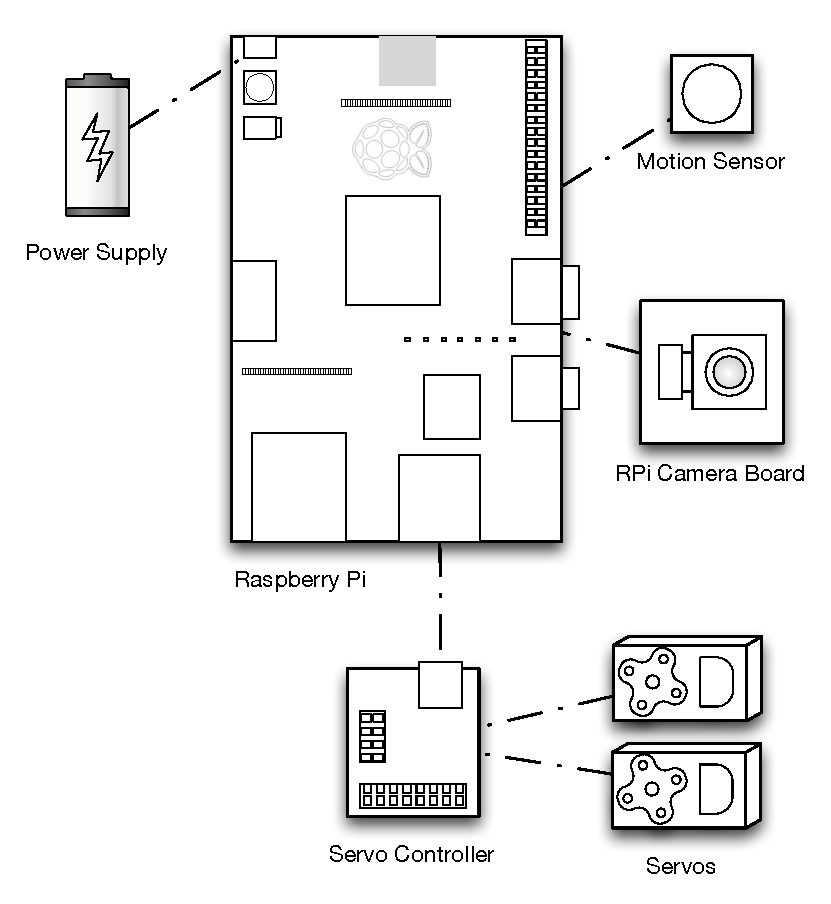
\includegraphics[width=0.6\textwidth]{graphs/rpi_1.pdf}
\caption{Connected hardware for computer vision component of project. It includes a power supply, motion sensor, RPi camera board, servo controller and two servos.}
\label{fig:cvhardware}
\end{figure}


The first \rpi\xspace will be responsible for subject tracking via computer vision. It will detect the subject via an attached camera and communicate directly with a servo controller to move the microphone mount. In an effort to conserve power, this \rpi\xspace will also have a motion sensor connected to one of its General Purpose Input/Output (GPIO) ports. When no motion is detected, it will power down the connected peripherals. Figure \ref{fig:cvhardware} illustrates the connected components for this device.


\begin{figure}
\centering
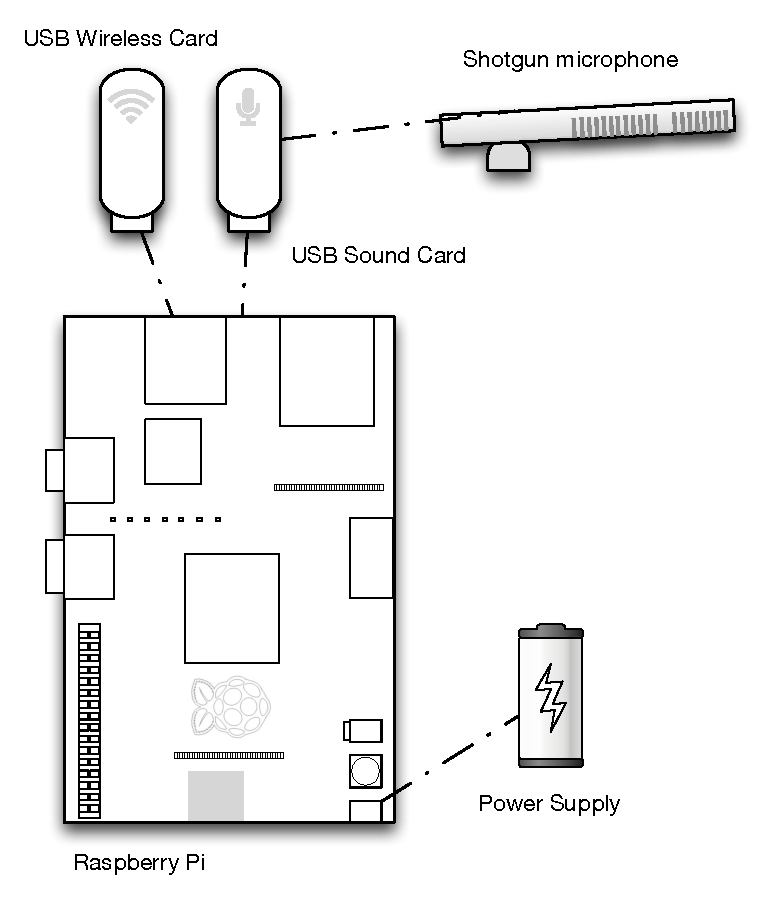
\includegraphics[width=0.6\textwidth]{graphs/rpi_2.pdf}
\caption{Connected hardware for audio recording component of project. It includes a power supply, sound card, shotgun microphone and wireless card.}
\label{fig:audiohardware}
\end{figure}

The second \rpi\xspace will be responsible for the audio recording and processing. It will be connected to a shotgun microphone attached for direction recording with minimal noise interference. An addition USB sound card will also included to support the recording. The intention is to also perform voice-to-text processing through a web service, so a wireless card will also be attached for communication with the Interned. Figure \ref{fig:audiohardware} illustrates the connected components for this device.

Both \rpis\xspace will be networked together via the Ethernet ports for inter-device communication.

For a detailed summary of all involved hardware and its purpose in the project, see Table \ref{table:hardwaretable}. 


%\begin{figure}
%        \centering
%        \begin{subfigure}[b]{0.5\textwidth}
%                \centering
%                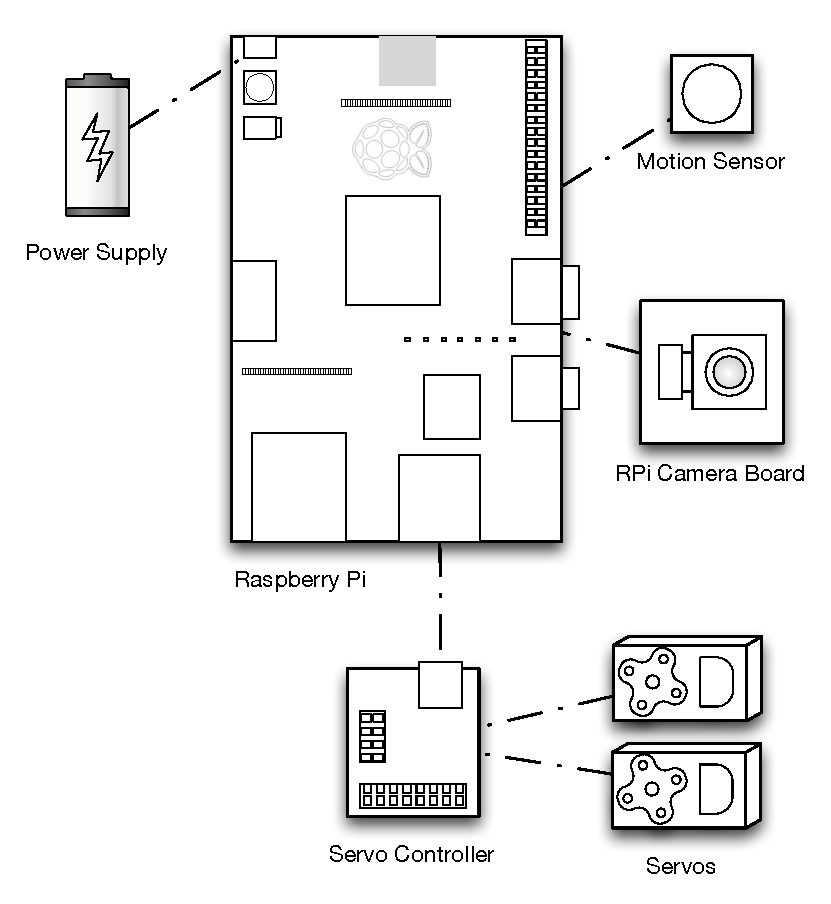
\includegraphics[width=\textwidth]{graphs/rpi_1.pdf}
%                \caption{Computer vision}
%                \label{fig:vision}
%        \end{subfigure}%
%        \begin{subfigure}[b]{0.5\textwidth}
%                \centering
%                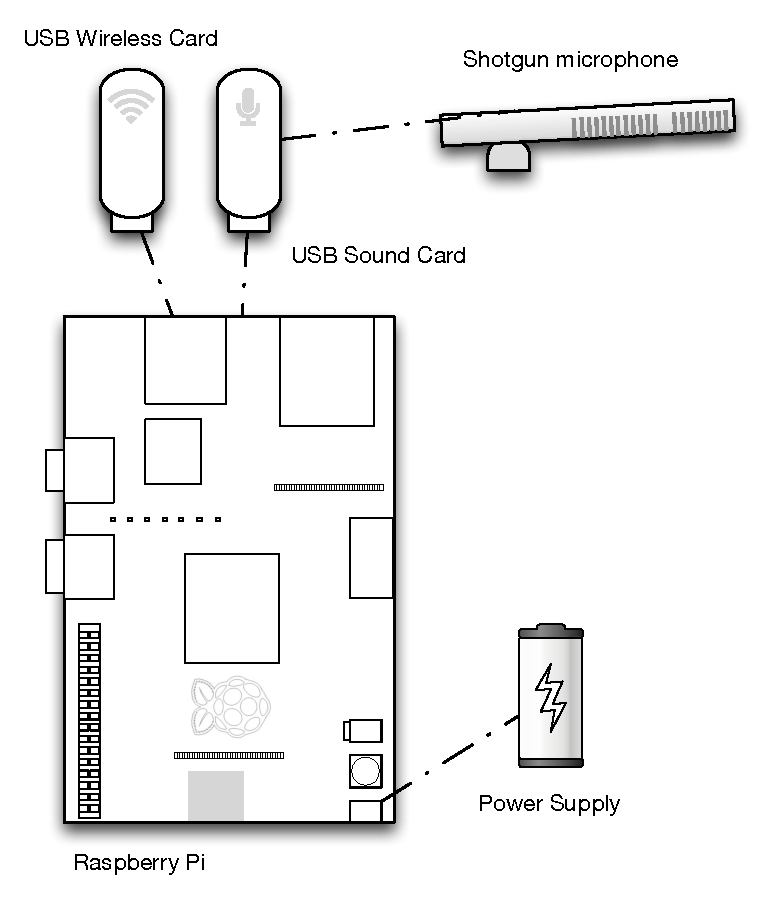
\includegraphics[width=\textwidth]{graphs/rpi_2.pdf}
%                \caption{Sound recording}
%                \label{fig:sound}
%        \end{subfigure}
%        \caption{Connected hardware setup for the project. Each \rpi\xspace has a dedicated task of computer vision or sound recording.}\label{fig:hardware}
%\end{figure}



\begin{center}
\begin{table}
\begin{tabular}{ |l|c|p{6cm}| }
    \hline
    
    Hardware & Quantity & Purpose \\ \hline
    
    \rpi & 2 & Due to the inherent complexity of audio and video processing, the solution workload will be split across two \rpis. The first will handle the computer vision and controlling the servos. The second is for processing audio and data storage.\\ \hline

    Camera & 1 & Either a RPi Camera board or USB web cam will be used for subject tracking through computer vision. \\ \hline
    
    Servos & 2 & Two servos will be used to control the microphone mount. One servo will manoeuvre the mount on an X axis, while the other is used for the Y axis. \\ \hline
        
    USB servo controller & 1 & This will be used to improve the movement accuracy of the servos \\ \hline
    
    USB sound card & 1 & The \rpi\xspace has no in-built audio input jack, so an external sound card will be used to facilitate connecting the microphone. \\ \hline
    
    
    Shotgun microphone & 1 & This microphone will give us targeted audio for recording voice and minimising background noise. \\ \hline
    
    
    Motion sensor & 1 & To conserve battery before and after a recording session, a low-power motion sensor will be used to detect the presence of a subject in the room. The solution will return to "standby mode" if no movement is detected.\\ \hline

    Power supply & 2 & To take advantage of the lightweight nature of the \rpi\xspace and components, an external battery pack will be used to make the solution portable.\\ \hline


    Wireless card & 1 & The voice-to-text processing will be performed remotely, so an unobtrusive internet connection will be required.\\ \hline
    
\end{tabular}
\caption{Summary of hardware}
\label{table:hardwaretable}
\end{table}

\end{center}

\section{Design Considerations}

CPU usage. Power consumption. Storage capability for prolonged usage. Modularity of components/


\subsection{Goals and Objectives}

This project aims to provide an easy way to audio record and annotate lectures, talks and other presentations. The platform is to be relatively portable, require minimal setup and start-up time...

\subsection{Assumptions and Dependencies}

...

\subsection{General Constraints}

...

\subsection{Development Methodology}

...

\section{Architecture}

...

\subsection{System Design}

...

\subsection{Data Design}

...

\subsection{Program Design}

...

\subsubsection{Detailed Module Design}

...


\section{Testing Issues}

...

\subsection{Types of Testing to be conducted}

...

\subsection{Performance Bounds}

...




\section{Roles and Responsibilities}

Due to an unfortunate circumstance, our final group didn't form until week four. As a result there is cross-overs in our teams individual strengths. The roles have been divided with some shared responsibilities for delivering the final solution. All three group members will be writing software and experiment with hardware.


\subsection{Val Lyashov}
\textit{Val} has been working with computer components since he was 16. He will take on the role of designing the hardware solution and providing the operating environment. He will also be responsible for drafting communication interfaces to the hardware in Python, which will later be ported to C by the other members.


\subsection{"Alfred" Yang Yuan}
\textit{Alfred} is an experienced programmer who has professionally worked with C++ for over 3 years. He will be responsible for the final software architecture and optimisation of the software layer. His role will also involve improving the scripts written by the other team members to be multi-threaded and run efficiently with the hardware.

\subsection{Neil Ang}
\textit{Neil} has strong programming background and a particular interest in intelligent system design. He will be responsible for implementing the object tracking and network communication between multiple \rpis. He will also take on the responsible for the technical writing, and help the other team members with documenting the project. 



\section{Bibliography}

...



\end{document}